\documentclass[../revisedmain.tex]{subfiles}
\begin{document}
\paragraph{Slopes} It is useful and easy to find the rate of change for any point on a line. It is difficult to approximate how a curved function changes, however. Functions that aren't lines don't have defined slopes and we have to use a tangent line to find the slope at a point. It is difficult to find the tangent line at a point, so we must resort to finding secant approximations for the tangent line.
\begin{center}
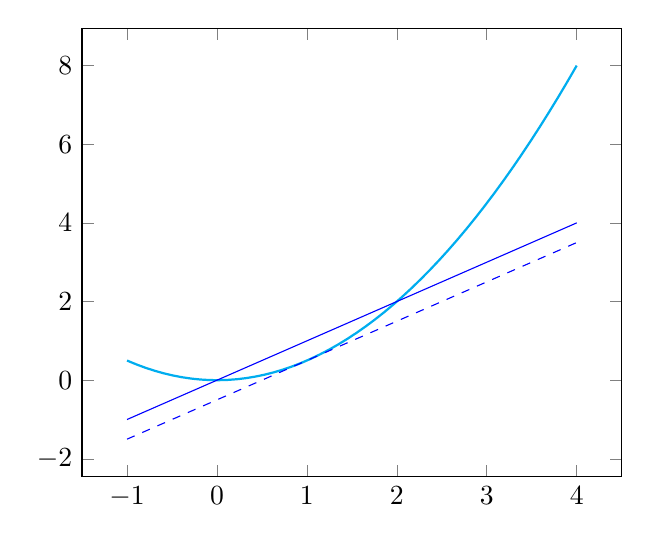
\begin{tikzpicture}
	\begin{axis}
	\addplot[domain=-1:4,cyan,thick,samples=50]{0.5*x^2};
	\addplot[domain=-1:4,blue,]{x};
	\addplot[domain=-1:4,blue,dashed]{x-0.5};
	\end{axis}
\end{tikzpicture}
\par The secant line $y=x$ approximates the dashed line tangent to the graph $f(x)=\frac{1}{2} x^2$ for the point $x=1$.
\end{center}
\end{document}